\begin{figure}[p]
\centering
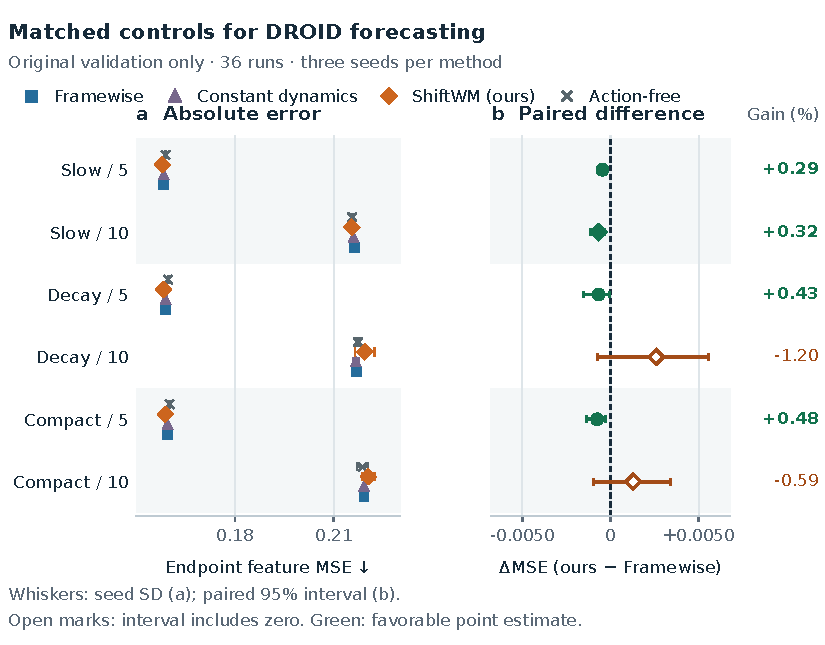
\includegraphics[width=\linewidth]{generated/real_video/generalization_summary.pdf}
\caption{\textbf{Matched optimization and capacity controls on original validation.} All 36 registered runs complete 30 epochs; selected checkpoints use the common all-five-query validation objective. Rows identify arm and forecast horizon in action blocks. Slow lowers learning rate, Decay increases weight decay, and Compact jointly reduces predictor/context capacity. (a) Equal-episode three-seed mean endpoint feature MSE with sample seed standard deviation; all four methods are shown. (b) ShiftWM (ours) minus matched Framewise with 95\% intervals from 10,000 paired session/seed bootstrap draws. Green positive reductions and open/filled interval markers distinguish point direction from interval exclusion of zero. The adjacent gain column is the relative MSE reduction, not the interval unit. Five and ten blocks include 141 and 141 eligible validation episodes, respectively. These exploratory development intervals are unadjusted for multiple comparisons; no additional held-out-test claim is made.}
\label{fig:generalization-summary}
\end{figure}
